\section{Wykorzystywane algorytmy}
W sekcji zostanie przybliżone działanie algorytmów(Rysunek \ref{fig:typy}) z uwzględnieniem znaczenia parametrów dobranych przez MetaOD.
Wszystkie algorytmy implementowane są z wykorzystaniem biblioteki \textit{Python Outlier Detection} (PyOD) \cite{zhao2019pyod}
\begin{figure}
    \centering
    \includegraphics[width=\textwidth]{chapters/istniejace/images/TypyAlgorytmów(1).png}
    \caption{Wykorzystywane algorytmy z podziałem na metodologię}
    \label{fig:typy}
\end{figure}

\subsection{OCSVM}
\textit{One-Class SVM} [Jednoklasowa maszyna wektorów nośnych] (OCSVM) \cite{ocsvm}. OCSVM jest binarną metodą klasyfikacji odwzorowującą dane wejściowe z wykorzystaniem funkcji jądrowej na przestrzeń wielowymiarową w poszukiwaniu hiperpłaszczyzny separującej poprawne obserwacje od anomalii.  
% Model jądrowy:
% \begin{equation}
%     f(x) = \sum_{i=1}^{N} \alpha _i y_iK(x_i,x)+b
% \end{equation}
% gdzie $K$ jest funkcją jądrową:
Funkcje jądrowe:
\begin{align*}
    Liniowa: x^Tx_i \\
    Wielomianowa: (\gamma x^Tx_i+c)^n \\
    RBF: exp(-\gamma ||x-x_i||^2) \\
    Sigmoidalna: tgh(\gammax^Tx_i+c)
\end{align*}
\label{eq:funjadro}

\subsection{kNN}
\textit{k-Nearest Neighbors}[Algorytym k najbliższych sąsiadów] (kNN) \cite{knn} opiera się na wnioskowaniu, że poprawne obserwacje będą w sąsiedztwie innych poprawnych obserwacji. Natomiast anomalie będą znacząco oddalone od klastrów normalnych obserwacji. Dla każdego elementu obliczamy metrykę do k = 1,...,N sąsiada. Wynik anomalności elementu zależy od metody (wybrana przez MetaOD):
\begin{itemize}
    \item \textit{largest} - anomalność punktu jest odległością do k-sąsiada (najdalej oddalonego)
    \item \textit{mean} - anomalność punktu jest średnią ze wszystkich odległości do sąsiadów
    \item \textit{median} - anomalność punktu jest medianą wszystkich odległości do sąsiadów
\end{itemize}

\subsection{LOF}
\textit{Local Outlier Factor}(LOF) \cite{lof} algorytm w odróżnieniu od algorytmu kNN rozpatruje lokalną gęstość względem sąsiadów. Podejście odnosi się do wad metod opartych na metryce (anomalie globalne) w przypadkach zbiorów danych o różnych gęstościach klastrów poprawnych obserwacji(Rysunek \ref{fig:anomalie_glob_lok}).
W celu obliczenia anomalności punktu należy dokonać 3 kroków:
\begin{enumerate}
    \item Dla rozpatrywanego punktu x, należy znaleźć k najbliższych sąsiadów
    \item Rozpatrując k najbliższych sąsiadów $N_k$, wyznaczyć zagęszczenie w k-sąsiedztwie punktu x obliczając \textit{local reachability density}(LRD): 
    \begin{equation}
        LRD_k(x) = 1/\Bigg(\frac{ \sum\limits_{o \in N_k(x)} d_k(x,o) }{|N_k(x)|}\Bigg)
    \end{equation}
    gdzie $d_k(\cdot)$ oznacza \textit{reachability distance}
    \item Ostatecznie obliczamy wartość LOF porównując LRD punktu $x$ z LRD k-sąsiada:
    \begin{equation}
        LOF(x) = \frac{ \sum\limits_{o \in N_k(x)} \frac{LRD_k(o)}{LRD_k(x)} }{|N_k(x)|}
    \end{equation}
\end{enumerate}
Wynik LOF jest stosunkiem
% współczynnikiem lokalnej gęstości.
Jeżeli wartość $LOF(x)>1$ oznacza to małą lokalną gęstość(anomalia lokalna). 
$LOF(x) \approx 1$ oznacza, że lokalna gęstość punktu x jest zbliżona do sąsiadów.

\subsection{COF}
\textit{Connectivity based Outlier Factor}(COF) \cite{cof} algorytm COF jest zbliżony do LOF, główną różnicą wybór k najbliższych sąsiadów (Rysunek \ref{fig:lcof}. LOF wybiera k najbliższych sąsiadów korzystając z odległości Euklidesowej, tworząc wokół analizowanego punktu sferę. COF tworzy zbiór k-sąsiadów dla punktu x wybierając najpierw najbliższego sąsiada dodając go do zbioru. Następnie wybiera punkt najbliższy do dowolnego elementu istniejącego zbioru k-sąsiadów do momentu aż zbiór będzie miał k elementów. Tworząc swojego rodzaju łańcuch k-sąsiadów. Obliczanie lokalnej gęstości przebiega w ten sam sposób co w LOF -- stosunek \textit{chaining distance} dla punktu x do średniej z \textit{chaining distance} dla k-sąsiadów :
\begin{equation}
    COF_k(x) = \frac{|N_k(x)| \cdot ac-dist_{N_K(x)}(x)}{\sum\limits_{o \in N_k(x)}ac-dist_{N_k(o))}(o)}
\end{equation}
gdzie $ac-dist_{N_k(x)}$ jest średnią odległością punktu x 
\begin{figure}
    \centering
    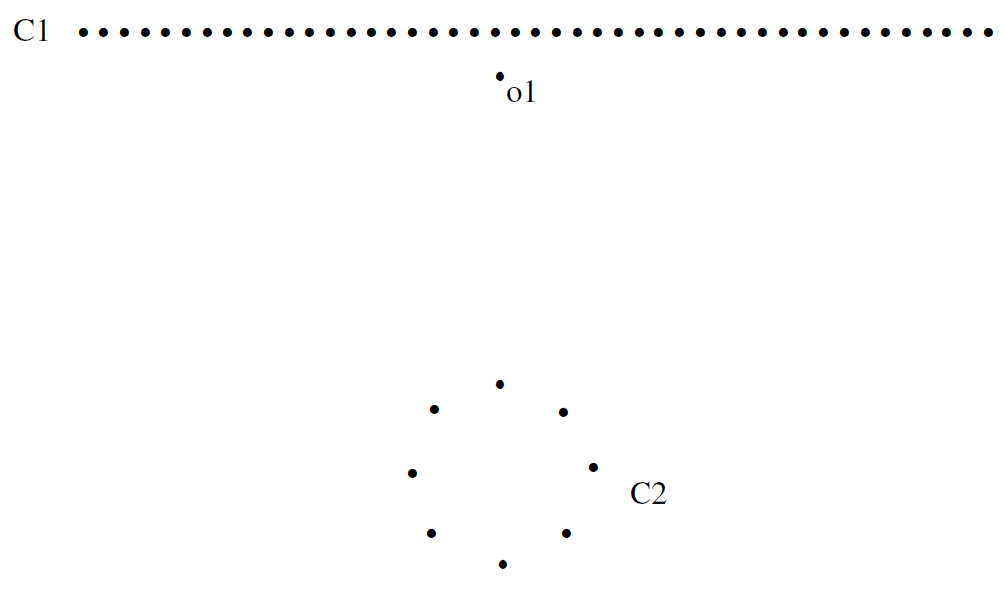
\includegraphics[width=.6\textwidth]{chapters/MetaOD/images/cof.png}
    \caption{Zbiór dla którego detekcja anomalii algorytmem LOF nie powiedzie się \cite{cof}}
    \label{fig:cof}
\end{figure}

\begin{figure}
    \centering
    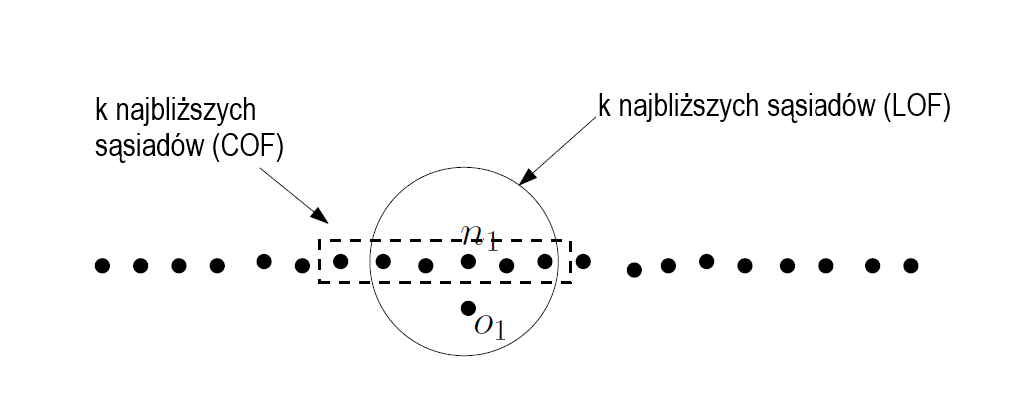
\includegraphics[width=.6\textwidth]{chapters/MetaOD/images/lvcof.png}
    \caption{Różnica w wyborze k najbliższych sąsiadów dla COF i LOF (k=5) \cite{chandola2009anomaly}}
    \label{fig:lcof}
\end{figure}

\subsection{ABOD}
\textit{Angel-based Outlier Detection}(ABOD) \cite{abod} W wielowymiarowych przestrzeniach kąty są stabilniejsze niż metryka, spowodowane jest to "przekleństwem wymiarowości". Rezultatem badań na temat zagadnienia "przekleństwa wymiarowości"\cite{curse} jest wniosek, że najdalszy punkt i najbliższy punkt zbiegają do 0 ze wzrostem wymiarów:
\begin{equation}
\lim_{d\to\infty} \frac{dist_{max} - dist_{min}}{dist_{min}} \longrightarrow 0
\end{equation}
Z tego powodu np. w grupowaniu dokumentów tekstowych jako miary podobieństwa wykorzystuje się miarę kosinusową \cite{huang2008similarity}. Algorytm ABOD zamiast metryki między punktami w sąsiedztwie porównuje kierunek wektorów skierowanych wychodzących z rozpatrywanego punktu $x$. Standardowy ABOD rozpatruje wszystkie punkty w zbiorze w odniesieniu do analizowanego punktu, jest to podejście o wysokiej złożoności obliczeniowej $O(n^3)$. W celu zmniejszenia złożoności obliczeniowej w pracy wykorzystamy FastABOD, który rozpatruje k-sąsiadów. Rysunek \ref{fig:abod} obrazuje założenie algorytmu ABOD, który do oceny anomalności punktu stosuje współczynnik \textit{Angle-based outlier factor}(ABOF):
\begin{equation}
    ABOF(x) = Var\frac{\langle \overrightarrow{xy}, \overrightarrow{xz} \rangle⟩}{\big\| \overrightarrow{xy\big\|}\big\| \overrightarrow{xz}\big\|},y,z \in B
\end{equation}
gdzie $B$ jest odpowiednio dobranym zbiorem, jako iż używamy FastABOD jest to zbiór k-sąsiadujących punktów. Czym niższy ABOF tym większe podejrzenie anomalii (PyOD w celu zachowania konwencji -- większa wartość wyjściowa algorytmu oznacza wyższą anomalność obserwacji -- stosuje przeciwność ABOF tzn. -ABOF)
\begin{figure}
    \centering
    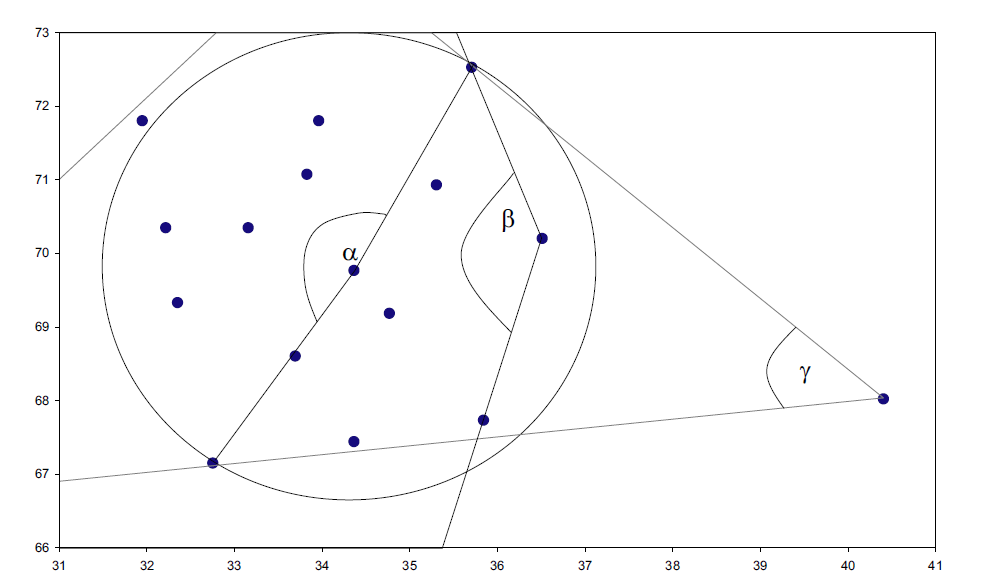
\includegraphics[width=.8\textwidth]{chapters/MetaOD/images/abod.png}
    \caption{Intuicja kierująca algorytmem ABOD \cite{abod}}
    \label{fig:abod}
\end{figure}

\subsection{HBOS}
\textit{Histogram-based Outlier Detection} (HBOS) \cite{hbos} zakłada liniową? niezależność cech. Określa anomalność punktu budując histogramy o n prostokątach

\subsection{LODA}
\textit{Lightweight Online Detector of Anomalies}(LODA) \cite{loda} wykorzystuje podejście budowania silnego klasyfikatora składającego się ze słabszych. Wykorzystuje histogram

\subsection{IForest}
\textit{Isolation Forest}(IForest) \cite{iforest} izoluje obserwacje wybierając losowo cechę i rozdzielającą ją na wartości maksymalne i minimalne coś na kształt drzewa, przez to że jest dużo drzew to mamy las. Odległość między korzeniem a liściem drzewa uśredniona pomiędzy wszystkie drzewa jest szukaną wartością anomalności obserwacji
\label{sub:IF}
